


\tikzset{every picture/.style={line width=0.75pt}} %set default line width to 0.75pt        

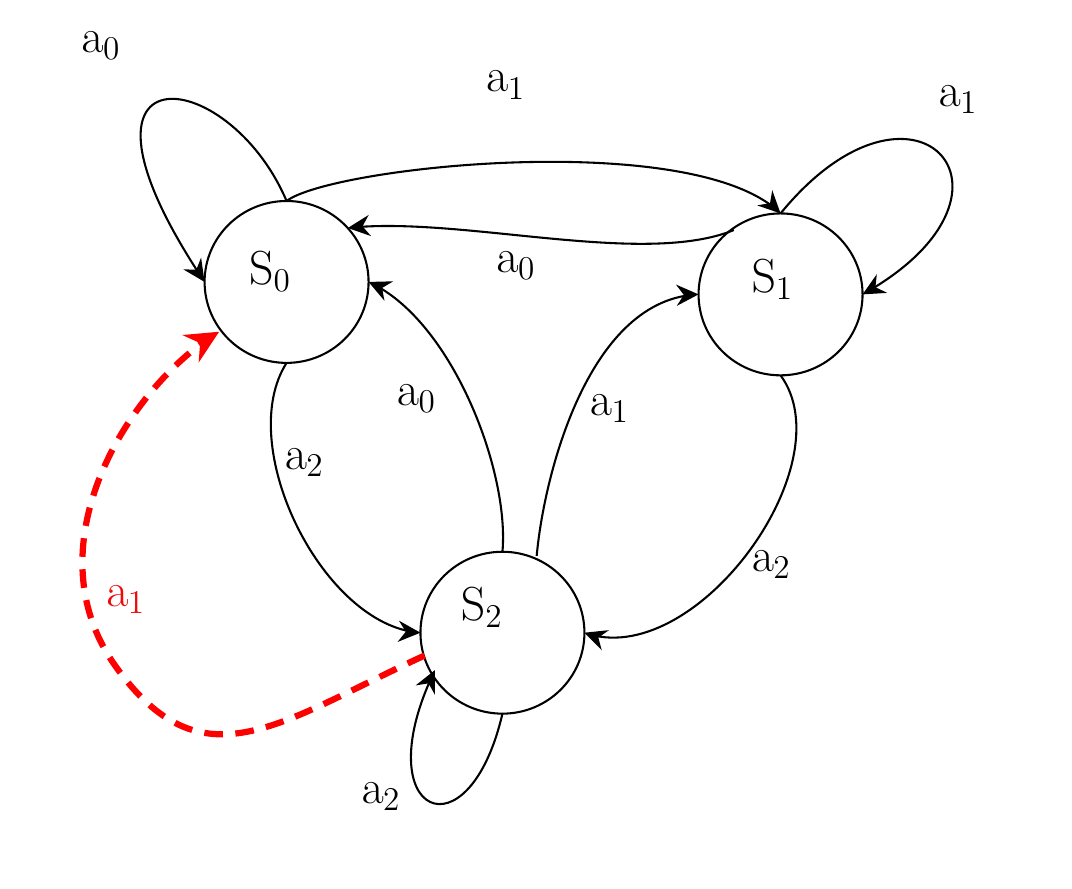
\begin{tikzpicture}[x=0.75pt,y=0.75pt,yscale=-1,xscale=1]
%uncomment if require: \path (0,457); %set diagram left start at 0, and has height of 457

%Shape: Ellipse [id:dp9438172929098625] 
\draw   (100,158) .. controls (100,136.46) and (117.68,119) .. (139.5,119) .. controls (161.32,119) and (179,136.46) .. (179,158) .. controls (179,179.54) and (161.32,197) .. (139.5,197) .. controls (117.68,197) and (100,179.54) .. (100,158) -- cycle ;
%Shape: Ellipse [id:dp4599560798398006] 
\draw   (204,327) .. controls (204,305.46) and (221.68,288) .. (243.5,288) .. controls (265.32,288) and (283,305.46) .. (283,327) .. controls (283,348.54) and (265.32,366) .. (243.5,366) .. controls (221.68,366) and (204,348.54) .. (204,327) -- cycle ;
%Shape: Ellipse [id:dp7447939409263706] 
\draw   (338,164) .. controls (338,142.46) and (355.68,125) .. (377.5,125) .. controls (399.32,125) and (417,142.46) .. (417,164) .. controls (417,185.54) and (399.32,203) .. (377.5,203) .. controls (355.68,203) and (338,185.54) .. (338,164) -- cycle ;
%Curve Lines [id:da5894404870673424] 
\draw    (139.5,119) .. controls (161.42,102.56) and (330.81,84.55) .. (375.54,123.19) ;
\draw [shift={(377.5,125)}, rotate = 224.65] [fill={rgb, 255:red, 0; green, 0; blue, 0 }  ][line width=0.08]  [draw opacity=0] (10.72,-5.15) -- (0,0) -- (10.72,5.15) -- (7.12,0) -- cycle    ;
%Curve Lines [id:da9289985657239253] 
\draw    (139.5,197) .. controls (114.51,236.2) and (155.43,320.55) .. (201.19,326.72) ;
\draw [shift={(204,327)}, rotate = 183.64] [fill={rgb, 255:red, 0; green, 0; blue, 0 }  ][line width=0.08]  [draw opacity=0] (10.72,-5.15) -- (0,0) -- (10.72,5.15) -- (7.12,0) -- cycle    ;
%Curve Lines [id:da12966817902715255] 
\draw    (243.5,288) .. controls (246.93,249.78) and (220.11,178.91) .. (181.39,159.15) ;
\draw [shift={(179,158)}, rotate = 24.23] [fill={rgb, 255:red, 0; green, 0; blue, 0 }  ][line width=0.08]  [draw opacity=0] (10.72,-5.15) -- (0,0) -- (10.72,5.15) -- (7.12,0) -- cycle    ;
%Curve Lines [id:da9803040408299597] 
\draw    (377.5,203) .. controls (408.53,245.36) and (338.17,343.01) .. (285.4,327.78) ;
\draw [shift={(283,327)}, rotate = 19.72] [fill={rgb, 255:red, 0; green, 0; blue, 0 }  ][line width=0.08]  [draw opacity=0] (10.72,-5.15) -- (0,0) -- (10.72,5.15) -- (7.12,0) -- cycle    ;
%Curve Lines [id:da8620836101311704] 
\draw    (139.5,119) .. controls (111.14,52.33) and (23.88,43.09) .. (98.86,156.28) ;
\draw [shift={(100,158)}, rotate = 236.2] [fill={rgb, 255:red, 0; green, 0; blue, 0 }  ][line width=0.08]  [draw opacity=0] (10.72,-5.15) -- (0,0) -- (10.72,5.15) -- (7.12,0) -- cycle    ;
%Curve Lines [id:da6425054933615544] 
\draw    (260,290) .. controls (263.45,251.58) and (284.36,168.54) .. (335.64,164.15) ;
\draw [shift={(338,164)}, rotate = 177.84] [fill={rgb, 255:red, 0; green, 0; blue, 0 }  ][line width=0.08]  [draw opacity=0] (10.72,-5.15) -- (0,0) -- (10.72,5.15) -- (7.12,0) -- cycle    ;
%Curve Lines [id:da6347469629611322] 
\draw    (377.5,125) .. controls (441.36,46.79) and (503.74,113.63) .. (419.59,162.52) ;
\draw [shift={(417,164)}, rotate = 330.89] [fill={rgb, 255:red, 0; green, 0; blue, 0 }  ][line width=0.08]  [draw opacity=0] (10.72,-5.15) -- (0,0) -- (10.72,5.15) -- (7.12,0) -- cycle    ;
%Curve Lines [id:da12627387672678436] 
\draw    (243.5,366) .. controls (227.17,436.29) and (178,415.43) .. (210.01,347.09) ;
\draw [shift={(211,345)}, rotate = 115.91] [fill={rgb, 255:red, 0; green, 0; blue, 0 }  ][line width=0.08]  [draw opacity=0] (10.72,-5.15) -- (0,0) -- (10.72,5.15) -- (7.12,0) -- cycle    ;
%Curve Lines [id:da08732909347306816] 
\draw    (355,133) .. controls (311.66,150.73) and (225.63,126.74) .. (171.45,131.75) ;
\draw [shift={(169,132)}, rotate = 353.66] [fill={rgb, 255:red, 0; green, 0; blue, 0 }  ][line width=0.08]  [draw opacity=0] (10.72,-5.15) -- (0,0) -- (10.72,5.15) -- (7.12,0) -- cycle    ;
%Curve Lines [id:da1623299464619441] 
\draw [color={rgb, 255:red, 255; green, 0; blue, 0 }  ,draw opacity=1 ][line width=2.25]  [dash pattern={on 6.75pt off 4.5pt}]  (206,338) .. controls (136,370) and (99,402) .. (57,343) .. controls (16.26,285.77) and (62.08,211.6) .. (103.2,184.39) ;
\draw [shift={(107,182)}, rotate = 149.24] [fill={rgb, 255:red, 255; green, 0; blue, 0 }  ,fill opacity=1 ][line width=0.08]  [draw opacity=0] (16.07,-7.72) -- (0,0) -- (16.07,7.72) -- (10.67,0) -- cycle    ;

% Text Node
\draw (120,142) node [anchor=north west][inner sep=0.75pt]  [font=\LARGE] [align=left] {S\textsubscript{0}};
% Text Node
\draw (362,146) node [anchor=north west][inner sep=0.75pt]  [font=\LARGE] [align=left] {S\textsubscript{1}};
% Text Node
\draw (222,304) node [anchor=north west][inner sep=0.75pt]  [font=\LARGE] [align=left] {S\textsubscript{2}};
% Text Node
\draw (191,206) node [anchor=north west][inner sep=0.75pt]  [font=\LARGE] [align=left] {a\textsubscript{0}};
% Text Node
\draw (39,36) node [anchor=north west][inner sep=0.75pt]  [font=\LARGE] [align=left] {a\textsubscript{0}};
% Text Node
\draw (239,142) node [anchor=north west][inner sep=0.75pt]  [font=\LARGE] [align=left] {a\textsubscript{0}};
% Text Node
\draw (452,62) node [anchor=north west][inner sep=0.75pt]  [font=\LARGE] [align=left] {a\textsubscript{1}};
% Text Node
\draw (234,55) node [anchor=north west][inner sep=0.75pt]  [font=\LARGE] [align=left] {a\textsubscript{1}};
% Text Node
\draw (284,211) node [anchor=north west][inner sep=0.75pt]  [font=\LARGE] [align=left] {a\textsubscript{1}};
% Text Node
\draw (174,398) node [anchor=north west][inner sep=0.75pt]  [font=\LARGE] [align=left] {a\textsubscript{2}};
% Text Node
\draw (137,237) node [anchor=north west][inner sep=0.75pt]  [font=\LARGE] [align=left] {a\textsubscript{2}};
% Text Node
\draw (362,286) node [anchor=north west][inner sep=0.75pt]  [font=\LARGE] [align=left] {a\textsubscript{2}};
% Text Node
\draw (51,303) node [anchor=north west][inner sep=0.75pt]  [font=\LARGE,color={rgb, 255:red, 238; green, 10; blue, 10 }  ,opacity=1 ] [align=left] {a\textsubscript{1}};


\end{tikzpicture}
